\documentclass[]{article}


\usepackage{tikz}
\usepackage{graphicx}
\usepackage{rotating}
\frenchspacing

\begin{document}

\title{Voorstel uitwerking}
\author{Axel Faes \and Matthijs Kaminski}
\date{4 februari 2015}
\maketitle

\section{Inleiding}
We hebben een voorstel uitgewerkt voor de visuele programming IDE.  Ons voorstel is nog steeds event-based. In dit voorstel wordt uitgelegd wat we precies zien als events alsook de sprites en onderlinge samenhang. Er is een methode voor parameter passing ingevoegd. Er wordt verwacht dat de gebruiker een kleine voorkennis heeft m.b.t. logica. Achteraan het verslag zit een uitgewerkt voorbeeld.  \\\\ 
De opgelegde eisen zoals de professionele look, multi-language, opslaan is een leesbaar data formaat blijven uiteraard nog steeds gelden in dit voorstel. Ook de voorbeelden die eerder besproken zijn kunnen uitgewerkt worden in de omgeving van het nieuwe voorstel.
\section{Events}
\subsection{Wat stelt een event voor?}
Om onderlingen communicatie tussen sprites voor te stellen, gebruiken we een event. Een event kan al dan niet een message bevatten. Een event zonder message kan beschouwd worden als een trigger. Een message kan beschouwd worden als een struct. Een message kan meerdere primitieve types bevatten (int, string of boolean). Met elke variable in de message wordt een naam geassocieerd. Deze kan gebruikt worden om de variabele te accessen. Ook met het event zelf moet een ID hebben die als type geldt. De gemaakte events zijn dan verder in de IDE beschikbaar.\\\\
Het zenden van een event door een sprite noemt een broadcast. Naar welke andere sprites het event wordt verzonden, kan worden bepaald in het wired-view van het canvas.

\subsection{Visuele voorstelling: Wired-view van het canvas.}
\label{Visuele voorstelling: Wired-view van het canvas.}
Er is een aparte view waarin alle instanties van sprites als blokjes getoond worden. Deze blokjes bevatten inkomende en uitgaande poorten. Deze stellen respectievelijk de evenementen voor die de sprite wil ontvangen en de evenementen die het uitzendt. Er kunnen verbindingen gemaakt worden tussen de uitgaande poorten van een sprite en de inkomende poorten van een andere sprite.\\\\ 
Dit aparte view is echter de begin positie van alle gewenste instanties van de aangemaakte sprites. De gebruiker heeft de optie om de verbindingen al dan niet te tonen. Voor de debug-modus zou dit view statisch zijn. Terwijl een extra view het eventueel bewegen van de sprites toont. De gebruiker kan zo de flow van events bekijken.

\subsection{Creatie events}
Nieuwe events kunnen aangemaakt worden door de gebruiker in een aparte sectie van de IDE. Een event moet een type hebben, vervolgens kan een message (data) meegegeven worden aan dit event. Deze message is een POD (plain old data) die opgebouwd word door de gebruiker. Hierin zal elke variable een unieke naam en specifiek type hebben. Het doorgeven van events door/aan specifieke instanties werd beschreven in \ref{Visuele voorstelling: Wired-view van het canvas.}. \\\\ 
\begin{figure}
  \centering
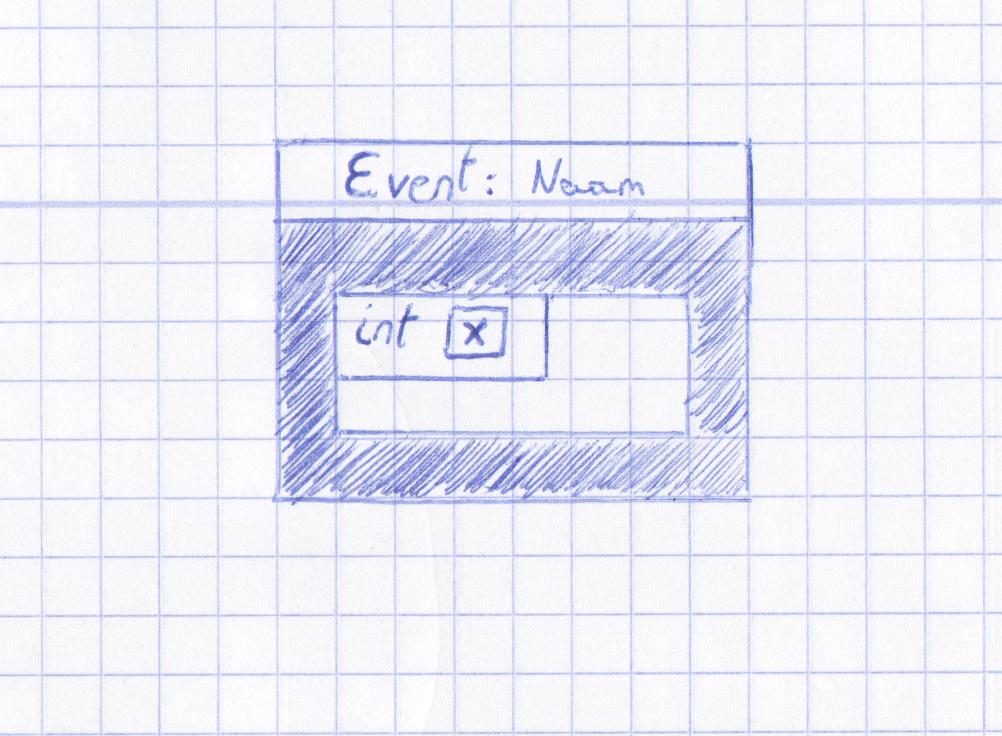
\includegraphics[scale=0.20]{mockups/eventcreatie.jpg}
  \caption{Creatie van events.} \label{eventcreatie}
\end{figure}

\subsection{Standaard events}
Er zijn standaard events beschikbaar zoals oa. onKeyPress, onClicked, onStart, enz. Deze events zijn nuttig om interactie te hebben met het visuele canvas.  
\section{In een sprite}
\subsection{Gebruiken van events waarop een sprite is geabonneerd}
Een sprite kan zich abonneren op events. Dit werd besproken \ref{Visuele voorstelling: Wired-view van het canvas.}. Het afhandelen van een event gebeurt door een handler die het event binnen krijgt. Het raadplegen van de inhoud van een event, kan doormiddel van een accesblok. Zoals beschreven in het voorbeeld \ref{Voorbeeld}.
\subsection{Verzenden van events}
Een sprite kan events broadcasten. Dit kan met behulp van een broadcast blok. Hierin moet een event worden geplaatst. Als een event een message (data) bevat zal die message ook hier moeten worden ingevuld. \\\\
Een sprite zal ook een overzicht hebben met alle events die erdoor worden gebroadcast.
\subsection{Interne functie calls}
Een uitbreiding van visuele omgeving door toe te laten om functie calls te maken binnen een sprite. Eerst was het idee om dit voor te stellen met een lijn die twee nodes zou verbinden. Bij een Sprite met veel interne calls wordt dit echter onoverzichtelijk.\\\\
Figuur \ref{functiecalls} is een voorbeeld van een interne call. Een functie oproep van uit een andere functie. Dit zal worden voorgesteld door een pijl naar een kleine node. Deze node bevat de naam van de functie die zal worden opgeroepen. Alsook zijn input parameters. Hierin kunnen variable gebruikt worden die behoren tot de scope van de functie die deze functie respectievelijk oproept. Natuurlijk ook membervariabelen van de Sprite. De onderkant van een functieaanroep node bevat een leeg vakje voor de return waarde. Hierin steekt ook weer een variable die bij de scope van de functie behoort.\\\\
Bij het aanklikken van de functie aanroepblok zal duidelijk worden gemaakt waar de functie definitie zich bevindt.

\begin{sidewaysfigure}
  \centering
  
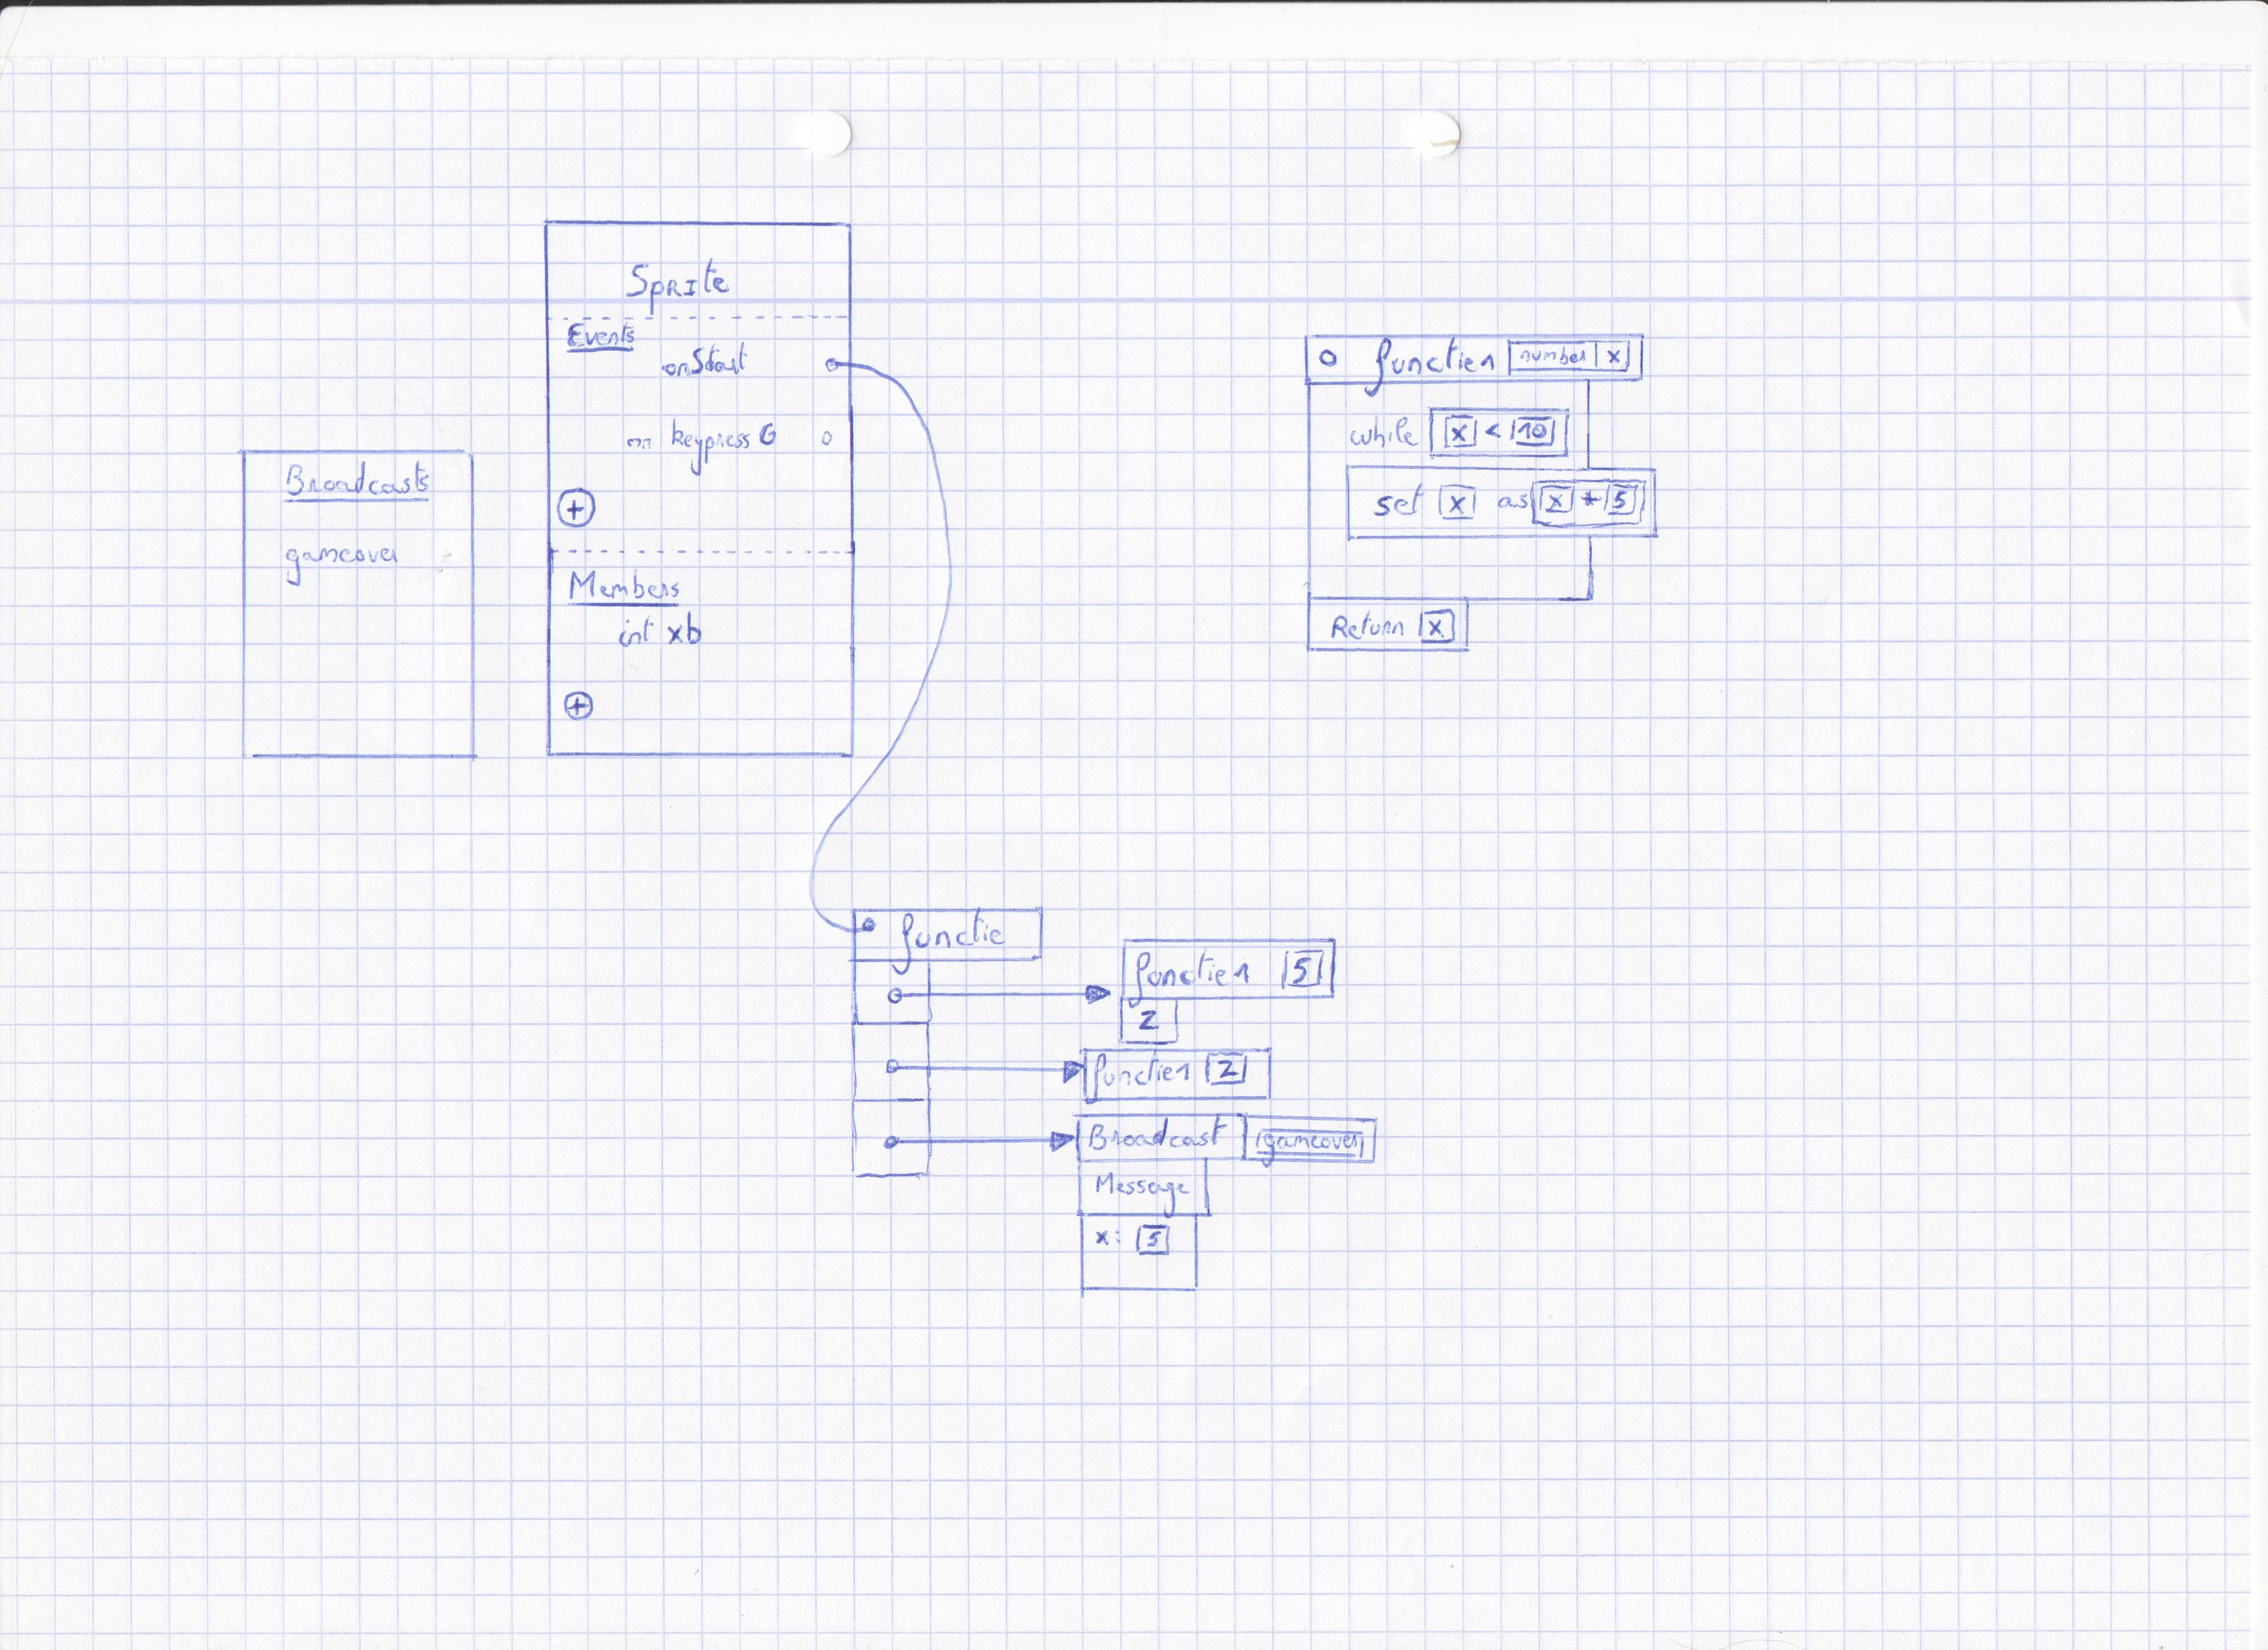
\includegraphics[scale=0.2]{mockups/functiecalls.jpg}
  \caption{Functiecalls.} \label{functiecalls}
\end{sidewaysfigure}

\subsection{Member variabelen}
Variabele die gelden per instance van een Sprite. Deze kunnen bijvoorbeeld de positie van de sprite in het canvas voorstellen.
\subsection{Visuele voorstelling van een sprite}
Er wordt een virtueel canvas en een console ge\"{i}mplementeerd. Een sprite kan dus al dan niet voorgesteld worden door een afbeelding.
 
 \section{Voorbeeld}
 \label{Voorbeeld}
 \subsection{Maken van het nodige event}
 \label{Maken van het nodige event}
 We maken een event van het type CallPhone aan. Dit type heeft als message \'{e}\'{e}n String variabele met als naam telnr. Dit maken gebeurt in het event gebeurt in het event creatie deel van de IDE. Hierna zal het event beschrikbaar zijn om te gebruiken in een sprite.
 \begin{figure}
  \centering
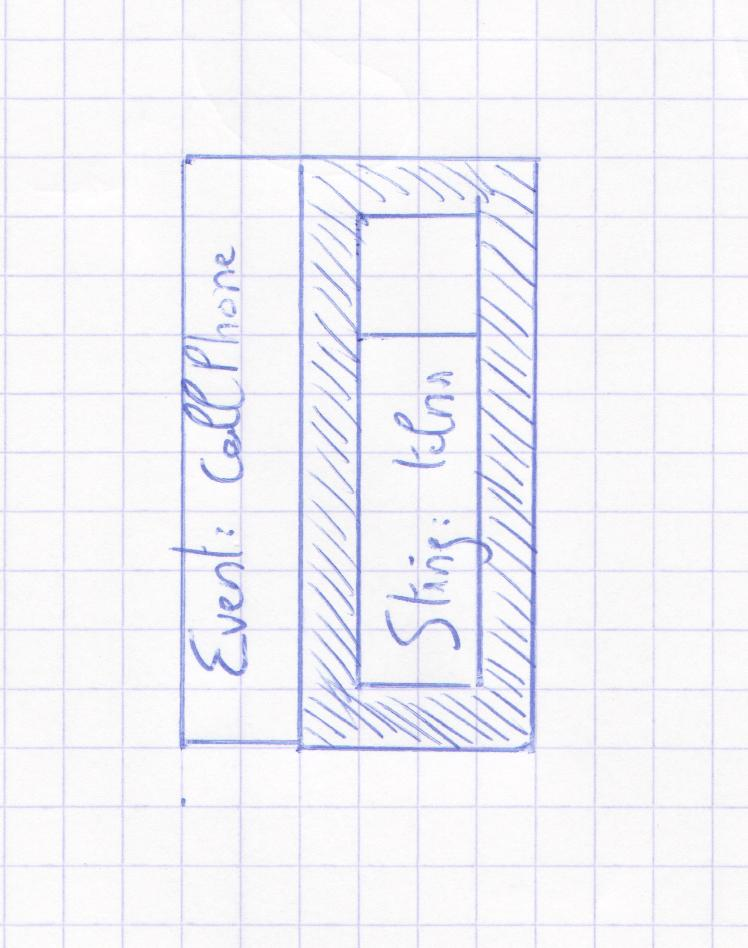
\includegraphics[scale=0.20]{mockups/callphone.jpg}
  \caption{Event CallPhone.} 
\end{figure} 
\subsection{Maken van de nodige Sprites} 
\subsubsection{Drukknop}
Een drukknop bezit over een standaard event onClick. Dit voegen we dus toe aan de input events van de sprite. Deze is verbonden met een handler genaamd Call deze broadcast de event CallPhone. Deze werd aangemaakt in \ref{Maken van het nodige event}.
 \begin{figure}
  \centering
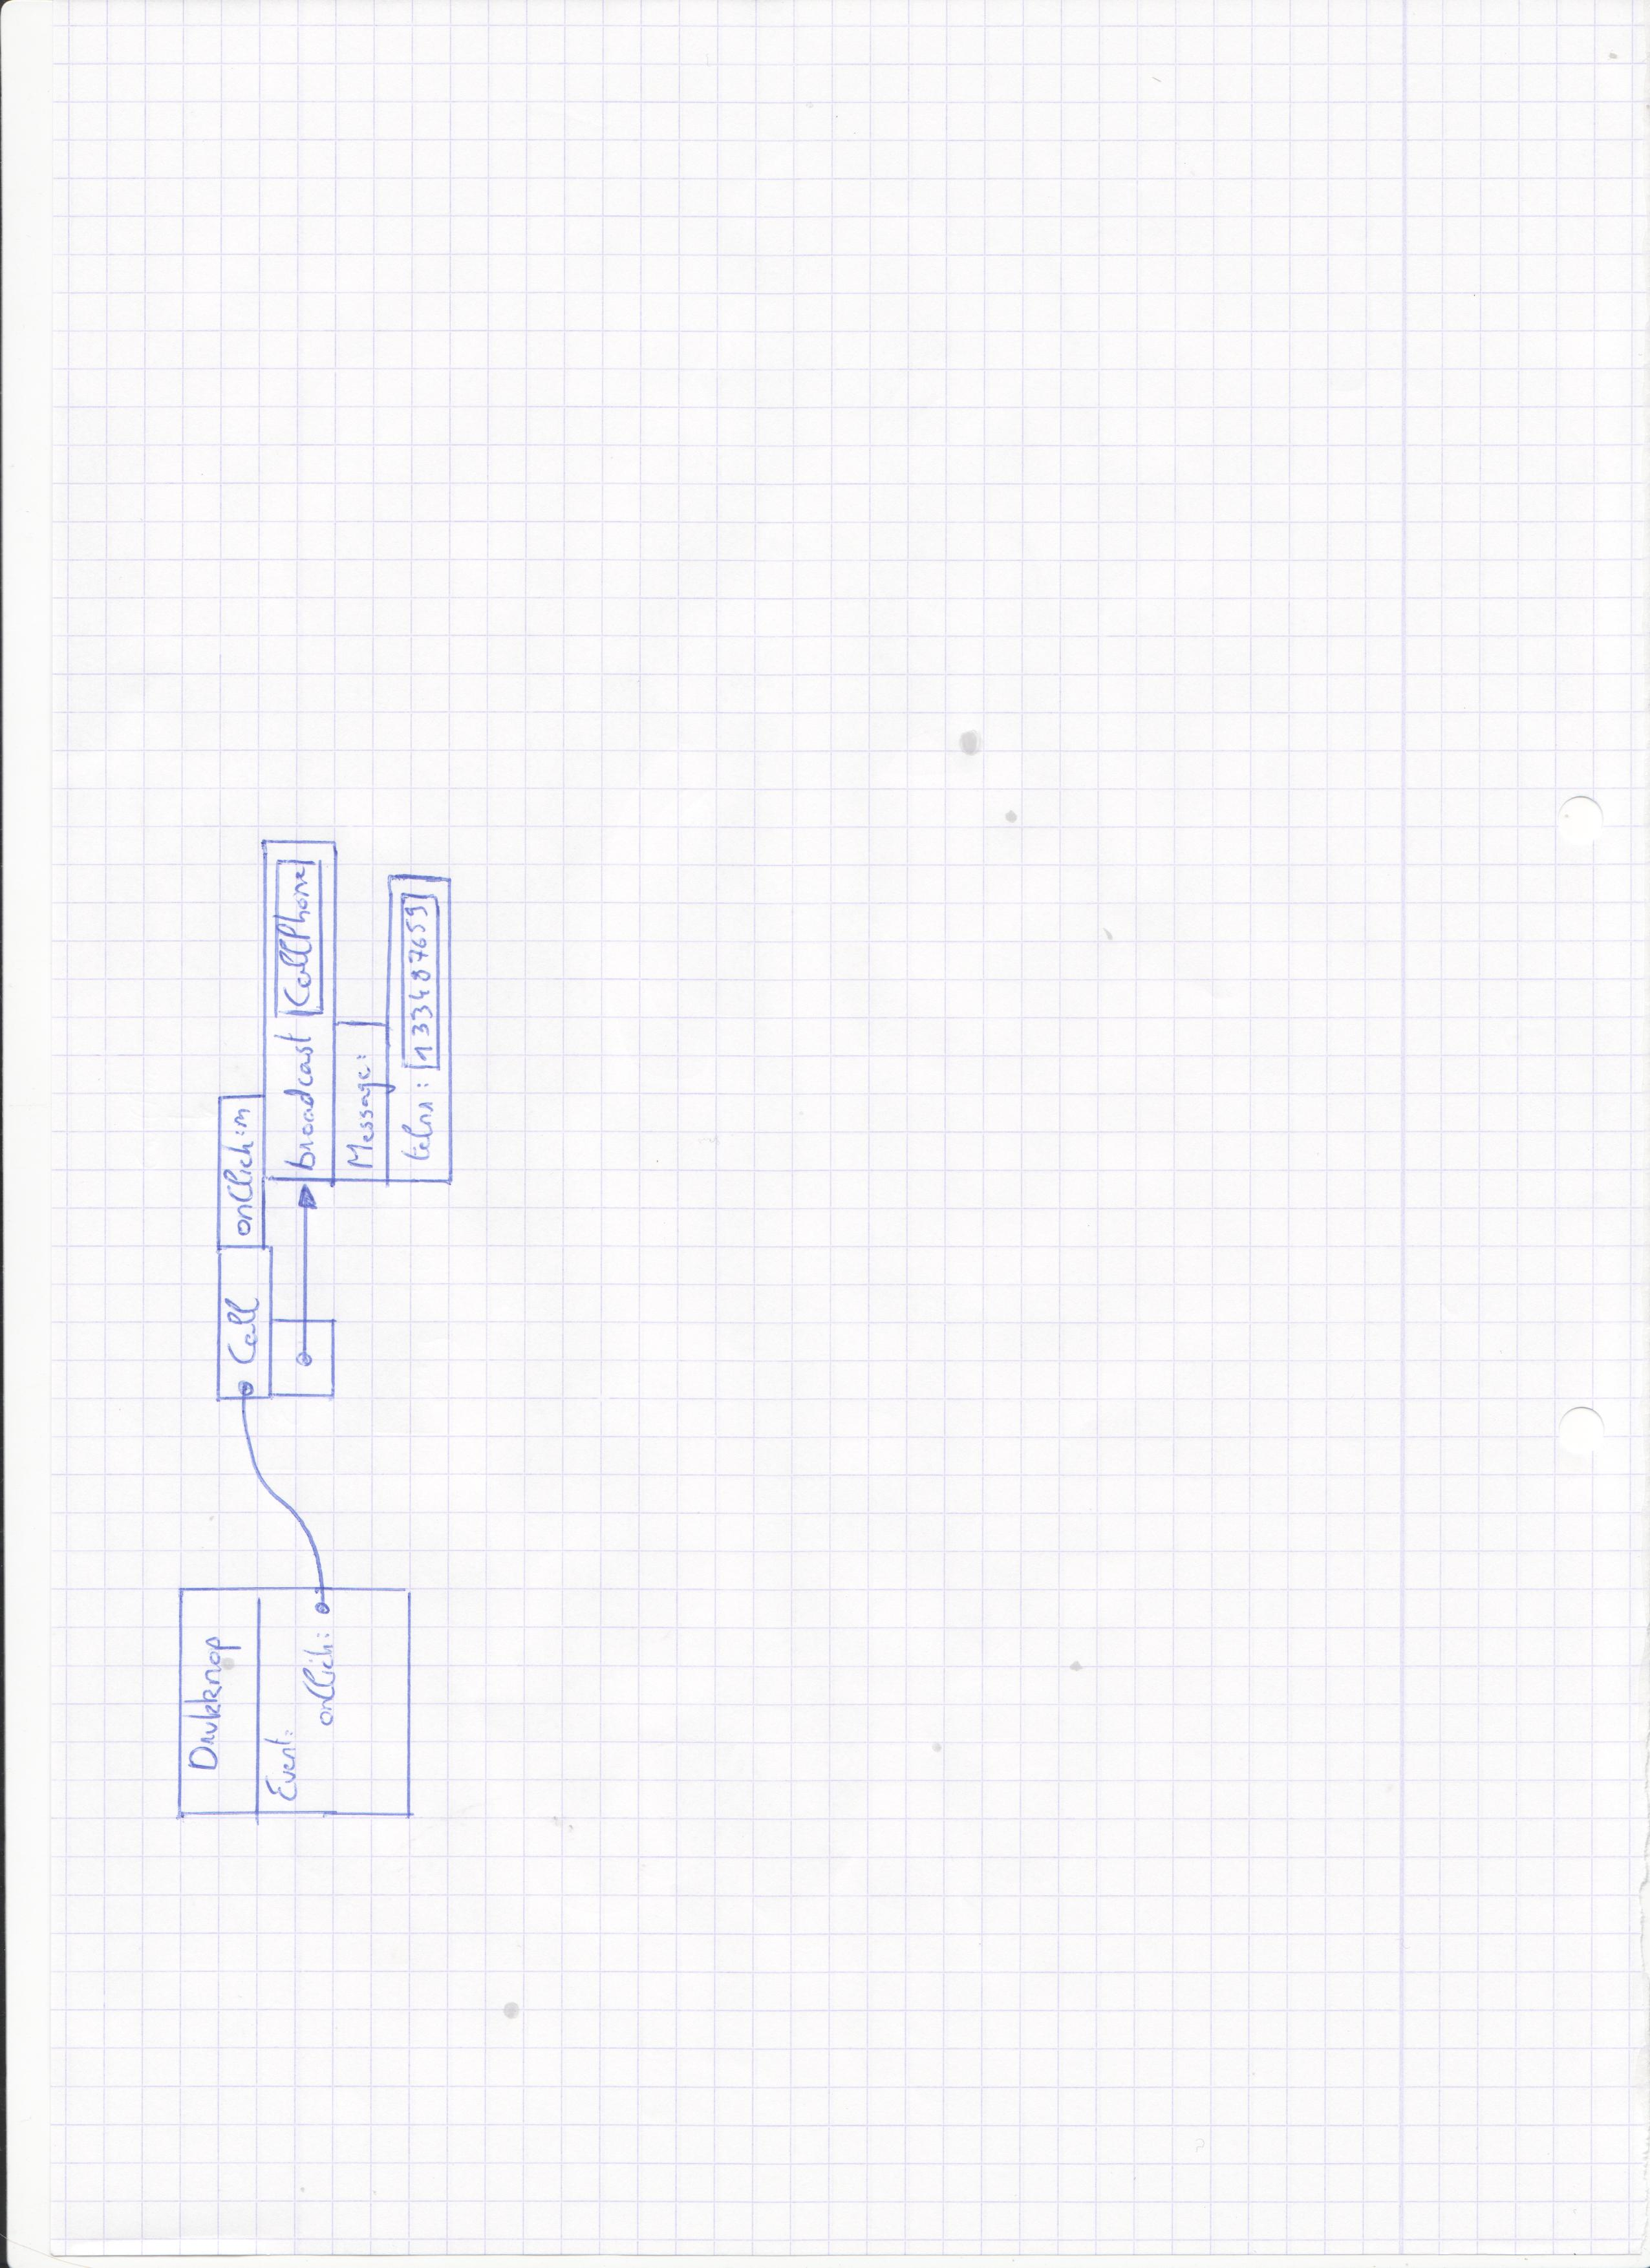
\includegraphics[scale=0.15]{mockups/drukknop.jpg}
  \caption{Drukknop.} 
\end{figure} 
\subsubsection{Telefoon}
Een telefoon bezit over een event CallPhone. Dit voegen we dus toe aan de input events van de sprite. Deze is verbonden met een handler genaamd Ringfunction. Deze handler heeft een parameter het event CallPhone die hij binnen krijgt door de oproep. De message (data) van dit event kan worden geaccessed door een acces blok zoals te zien in figuur \ref{telefoon}

 \begin{figure}
  \centering
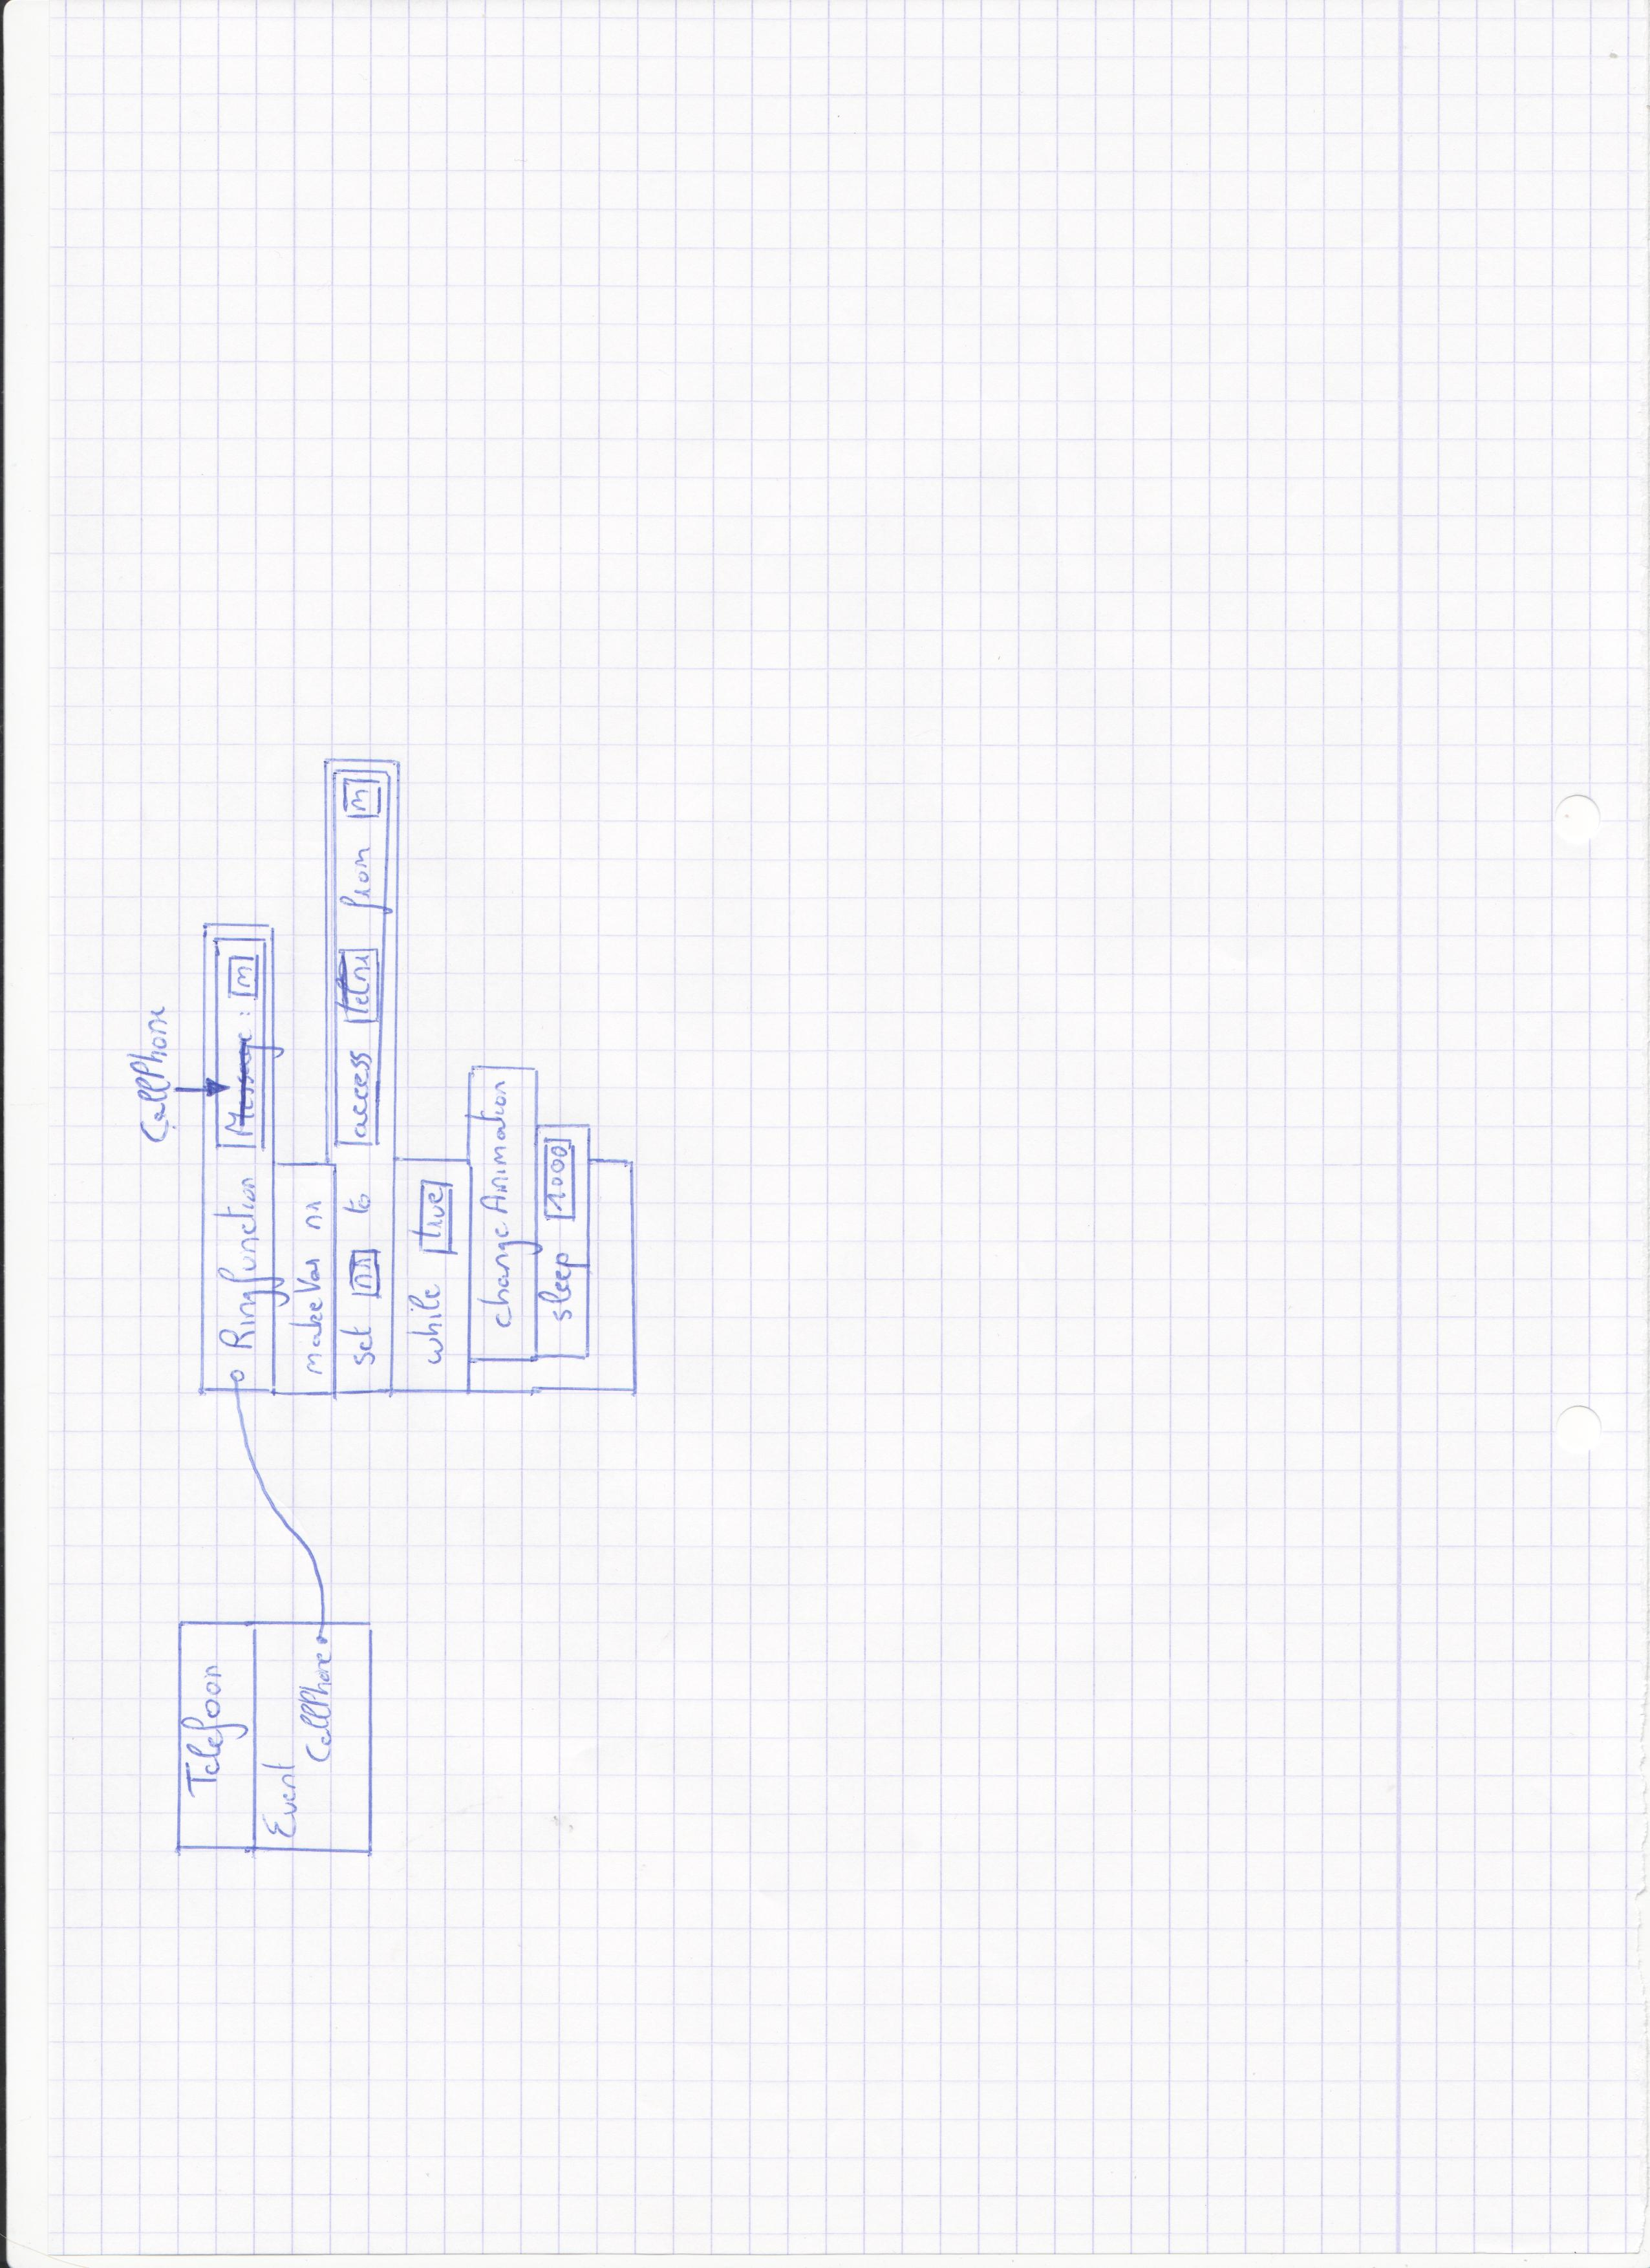
\includegraphics[scale=0.15]{mockups/telefoon.jpg}
  \caption{Telefoon.} \label{telefoon}
\end{figure} 

\subsection{Wired-view}
Het wired view bestaat uit vijf instanties. Er zijn drie drukknop instanties en twee telefoon instanties. De onderlinge verbindingen tonen aan hoe de gebroadcaste events verstuurt worden. Twee van de drukknoppen sturen hun gebroadcaste event CallPhone uit naar een unieke telefoon. De laatste drukknop stuurt de CallPhone event door naar alle telefoons. 
\begin{figure}
  \centering
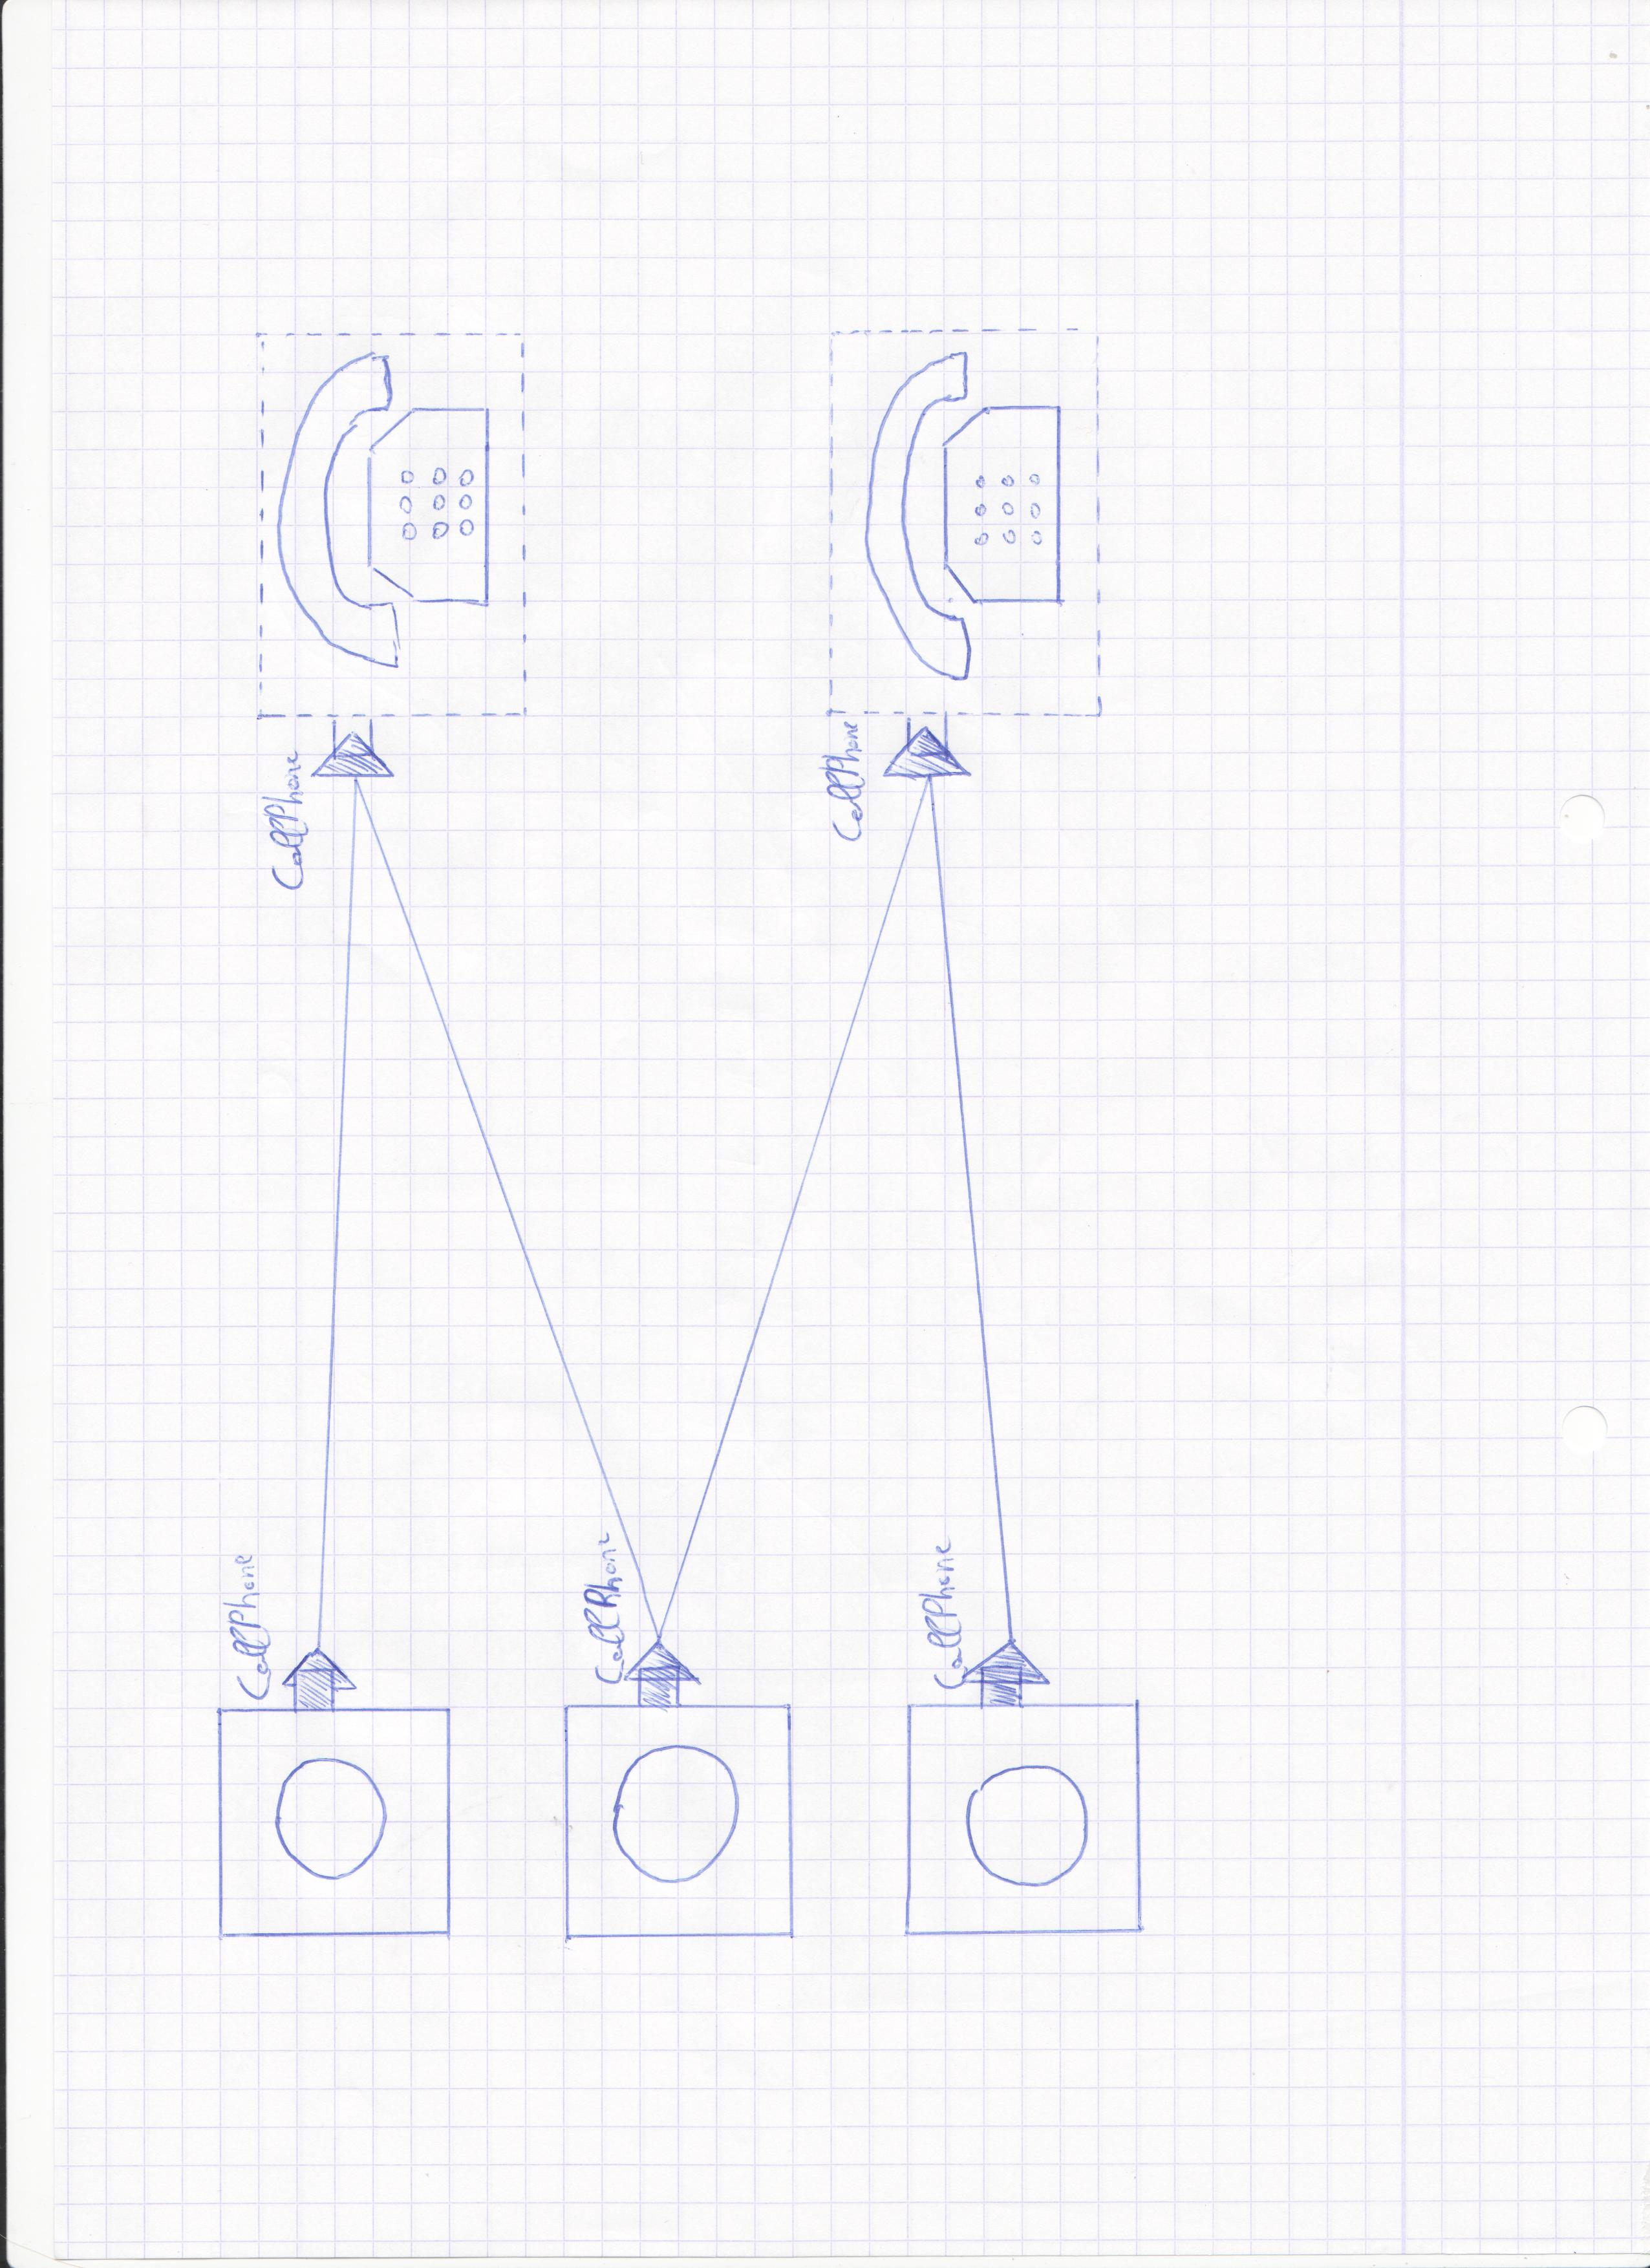
\includegraphics[scale=0.15]{mockups/wiredview.jpg}
  \caption{Wired-view.} \label{wire}
\end{figure}

\subsection{Canvas}
Bij het runnen van het programma zullen hierin de animaties van de telefoons getoond worden. En zal de gebruiker de input events kunnen uitvoeren.
\begin{figure}
  \centering
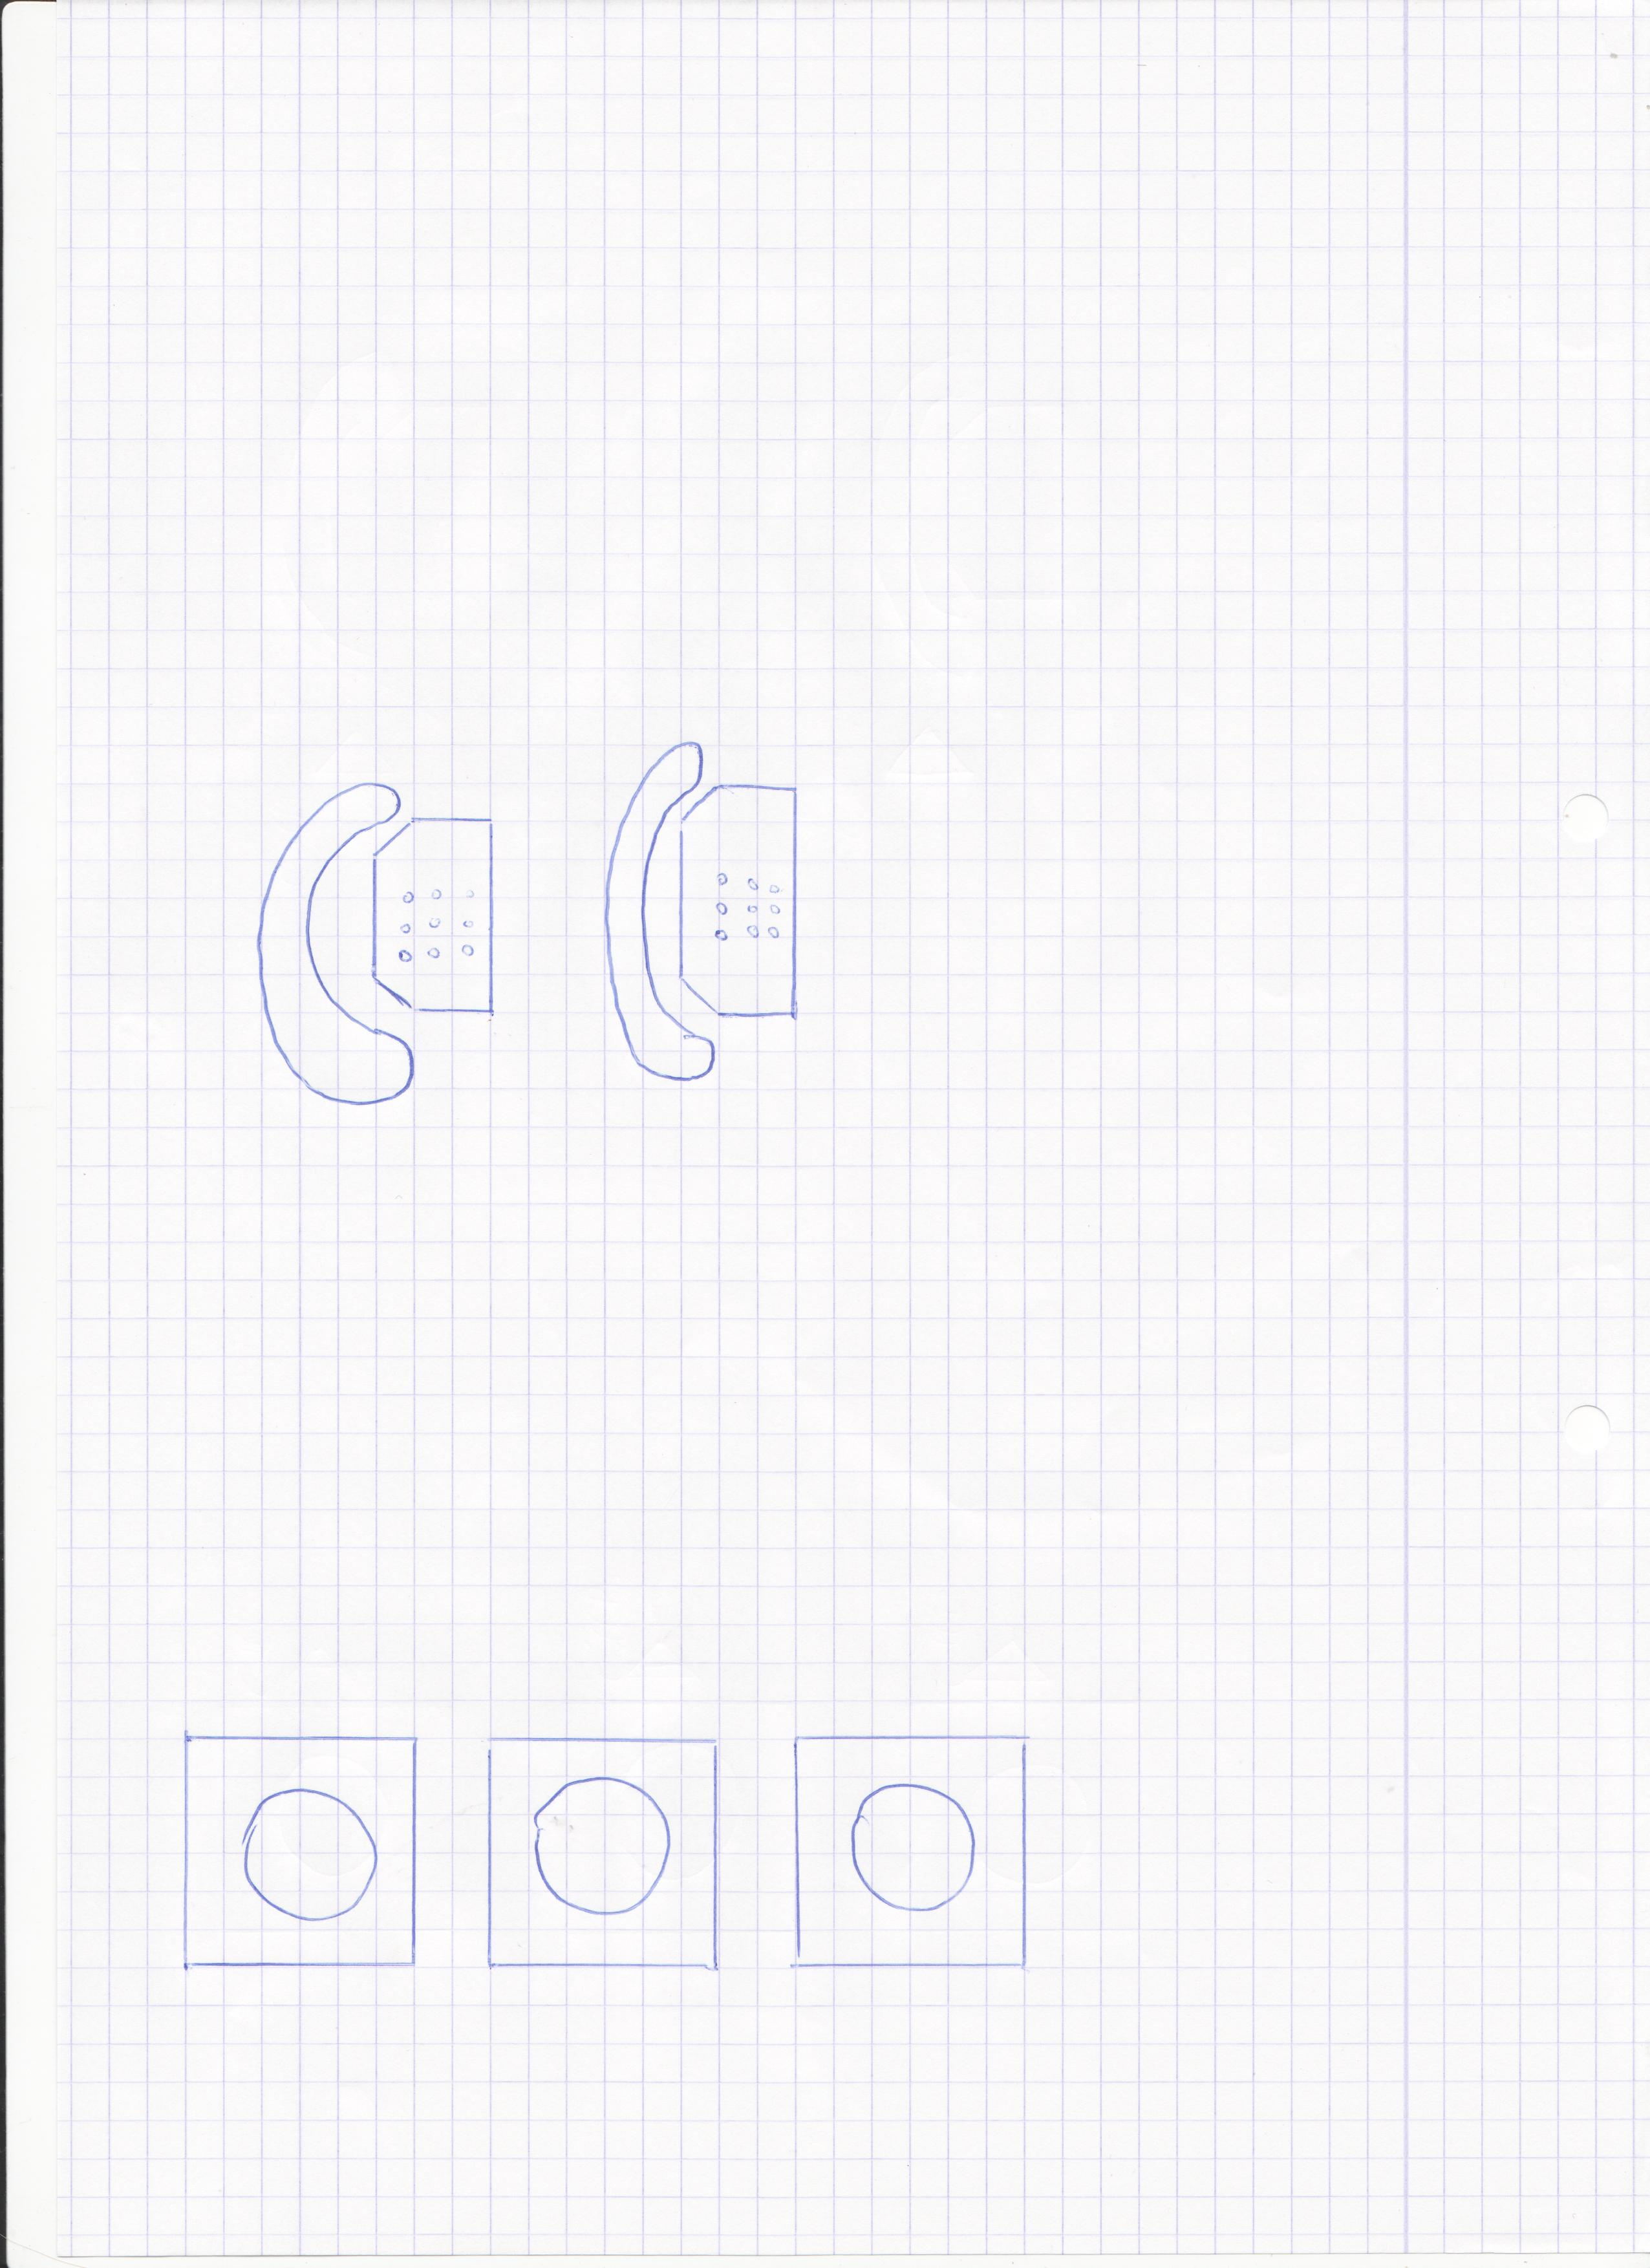
\includegraphics[scale=0.15]{mockups/canvas.jpg}
  \caption{Canvas.} \label{wire}
\end{figure} 


 

\end{document}